% Vorlage: https://www.pfsr.de/latex

% -- Anfang Präambel
\documentclass[german,  % Standardmäßig deutsche Eigenarten, englisch -> english
parskip=full,  % Absätze durch Leerzeile trennen
%bibliography=totoc,  % Literatur im Inhaltsverzeichnis (ist unüblich)
%draft,  % TODO: Entwurfsmodus -> entfernen für endgültige Version
]{scrartcl}

\usepackage[utf8]{inputenc}  % Kodierung der Datei
\usepackage[T1]{fontenc}  % Vollen Umfang der Schriftzeichen
\usepackage[ngerman]{babel}  % Sprache auf Deutsch (neue Rechtschreibung)

% Mathematik und Größen
\usepackage{amsmath}
\usepackage{amsfonts}
\usepackage[locale=DE,  % deutsche Eigenarten, englisch -> US
separate-uncertainty,  % Unsicherheiten seperat angeben (mit ±)
]{siunitx}
\usepackage{physics}  % Erstellung von Gleichungen vereinfachen

\usepackage{graphicx}  % Bilder einbinden \includegraphics{Pfad/zur/Datei(ohne Dateiendung)}

% Gestaltung
\usepackage{booktabs}  % schönere Tabellen
\usepackage[toc]{multitoc}  % mehrspaltiges Inhaltsverzeichnis
\usepackage{csquotes}  % Anführungszeichen mit \enquote
\usepackage{caption}  % Anpassung der Bildunterschriften, Tabellenüberschriften
\usepackage{subcaption}  % Unterabbildungen, Untertabellen, …
\usepackage{enumitem}  % Listen anpassen
\setlist{itemsep=-10pt}  % Abstände zwischen Listenpunkten verringern

% Manipulation des Seitenstils
\usepackage[headtopline = .5pt]{scrlayer-scrpage}

% Bibliographie
\usepackage[backend=biber]{biblatex}
\addbibresource{bibliography.bib}

% SI-Einheiten darstellen
\usepackage{siunitx}

% Tabellen mit geteilten Zeilen
\usepackage{multirow}

% Kopf-/Fußzeilen setzen
\pagestyle{scrheadings}  % Stil für die Seite setzen
\clearmainofpairofpagestyles  % Stil zurücksetzen, um ihn neu zu definieren
\automark{section}  % Abschnittsnamen als Seitenbeschriftung verwenden
\ofoot{\pagemark}  % Seitenzahl außen in Fußzeile
\ihead{\headmark}  % Seitenbeschriftung mittig in Kopfzeile

\usepackage[hidelinks]{hyperref}  % Links und weitere PDF-Features

% TODO: Titel und Autor, … festlegen

%\newcommand\norm[1]{\left\lVert#1\right\rVert} % Norm

\newcommand*{\titel}{Beschleunigermas­senspektrometrie und Methoden zur Altersbestimmung}
\newcommand*{\autor}{Sebastian Thiede, Alexander Lettau}
\newcommand*{\abk}{BM}
\newcommand*{\betreuer}{Dr. Johannes Lachner, Dr. Georg Rugel}
\newcommand*{\messung}{16.12.2021}
\newcommand*{\ort}{Helmholtz-Zentrum Dresden Rossendorf, DREAMS}

\hypersetup{pdfauthor={\autor}, pdftitle={\titel}}  % PDF-Metadaten setzen

% automatischen Titel konfigurieren
\titlehead{Praktikum des IKTP \abk \hfill TU Dresden}
\subject{Versuchsprotokoll}
\title{\titel}
\author{\autor}
\date{\begin{tabular}{ll}
Protokoll: & \today\\
Messung: & \messung\\
Ort: & \ort\\
Betreuer: & \betreuer\end{tabular}}

% -- Ende Präambel

\begin{document}
\begin{titlepage}
\maketitle  % Titel setzen
\tableofcontents  % Inhaltsverzeichnis setzen
\end{titlepage}

% ----- DOKUMENT ANFANG -----

\section{Aufgabenstellung}
Die Beschleunigermas­senspektrometrie (AMS) ist ein wichtiges Werkzeug zur Trennung und Detektierung von Nukliden.
Eine der häufigsten Anwendungen ist die Altersbestimmung von Proben aus der Natur durch Messung der Konzentration verschiedener Nuklide, die auf der Erdoberfläche durch kosmische Strahlung entstehen.
Im Gegensatz zu anderen Verfahren der Massenspektrometrie erreicht man bei der AMS eine sehr gute Unterdrückung atomarer und molekularer Isobare.
Die Messzeiten sind relativ kurz und es lassen sich auch kleine Proben untersuchen.

In diesem Versuch wurde der Beschleuniger DREAMS (DREsden AMS) vorgestellt.
Die generelle Handhabung wurde anhand folgender praktischer Aufgaben kennengelernt:
\begin{itemize}
  \item Inbetriebnahme eine Sputter-Ionenquelle und Erzeugung negativer Ionen
  \item Strahlentransport eines Isotopenpaares durch den Beschleuniger
  \item Kalibrierung der Verstärkung der gasgefüllten Ionistationskammer
  \item Aufnahme von Messwerten in der gasgefüllten Ionisationskammer
\end{itemize}

Zur Auswertung sind folgende Aufgaben zu bearbeiten:
\begin{itemize}
  \item Berechnung der Teilchenenergien nach dem Beschleuniger
  \item Plotten des Stromes des Ionenstrahls im Faraday Cup
  \item Abschätzung des Energieverlustes des Ionenstrahls in einer dünnen Folie
  \item Abschätzung des Energieverlustes des Ionenstrahls in Isobutan (Gas in der Ionisationskammer)
  \item Plotten der gemessenen Spektren und Identifikation der Ionen
  \item Berechnung der Konzentration von Radionukliden in einer unbekannten Probe
\end{itemize}

\section{Theorie}

\subsection{organische Szintillatoren}

Szintillatoren sind  Materialien die bei bestrahlung mit energiereichen Photonen oder geladenen Teilchen angeregt werden und die Anregungsenergie in Form von Licht wieder abgeben. Organische Szintillatoren bestehen wie der Name schon vermuten lässt vorwiegend aus Kohlenstoff, Wasserstoff, Sauerstoff und Stickstoff wie es auch in z.B. menschlichem Gewebe der Fall ist. Es liegt daher nahe Detektoren auf Basis organischer Szintillatoren für die Dosismessung im Strahlenschutz zu verwenden. Organische Szintillatoren bestehen typischerweise aus zwei Komponenten: Einem primären Fluoreszenzstoff (z.B. auf Basis von Polyvinyltoluol) und einem \glqq Wellenlängenschieber \grqq{} (z.B. POPOP) da die vom primären Fluoreszenzstoff abgegebenen UV-Strahlen in den meisten durchsichtigen Materialien eine nur sehr geringe Reichweite besitzen.

\subsection{Wechselwirkung von Photonen mit Materie}

Obwohl Photonen in vieler Weise mit Materie wechselwirken können sind für diesen Versuch nur zwei Prozesse von wesentlicher Bedeutung: Die Compton-Streuung und der Photoeffekt. In den folgenden Abschnitten werden beide näher erläutert.

\subsubsection{Photoeffekt}

Der Photoeffekt beschreibt die Anregung von Elektronen durch Absorption eines Photons.
Für den HPGe-Detektor ist vor allem der innere photoelektrische Effekt von Bedeutung. Er beschreibt die Zunahme der Leitfähigkeit eines Halbleiters durch Bildung von nicht aneinander gebundenen Elektron-Loch-Paaren. Der HPGe-Detektor besteht aus einem hochreinen Germanium-Kristall der zwischen einem $n^{+}$ Kontakt (typ. durch Lithium-eindiffusion) am positiven Spannungspol und einem $p^{+}$ Kontakt (typ. durch Bor-implantation) am negativen Spannungspol sitzt; Der Detektor insgesamt entspricht einer Halbleiterdiode in Sperrichtung. Trifft ein Photon auf den Detektor und erzeugt ein Elektron-Loch-Paar werden durch die anliegende Spannung Elektron und Loch abgesaugt und bilden so einen detektierbaren Verschiebungsstrom. Dafür muss das einfallende Photon natürlich genügend Energie besitzen um die Bandlücke zu überwinden (Für Germanium \SI{0.67}{\electronvolt}), praktisch jedoch deutlich mehr um das Siganl-Rausch-Verhältnis groß genug zu bekommen. So werden bei einfallenden Photonen von \SI{1}{\mega\electronvolt} etwa \num{3e5} Elektron-Loch-Paare erzeugt \cite{HPGe-Detektor}. Da bei Raumtemperatur eine ständige thermische Anregung der Elektronen enormes Signalrauschen verursachen würde ist eine Abkühlung mit flüssigem Stickstoff notwendig.
Für den zu kalibrierenden Detektor ist vor allem der äußere photoelektrische Effekt von Bedeutung, genauer für den Photoelektronenvervielfacher (Abb. \ref{theorie_PEV}).

\begin{figure}[ht]
	\centering
  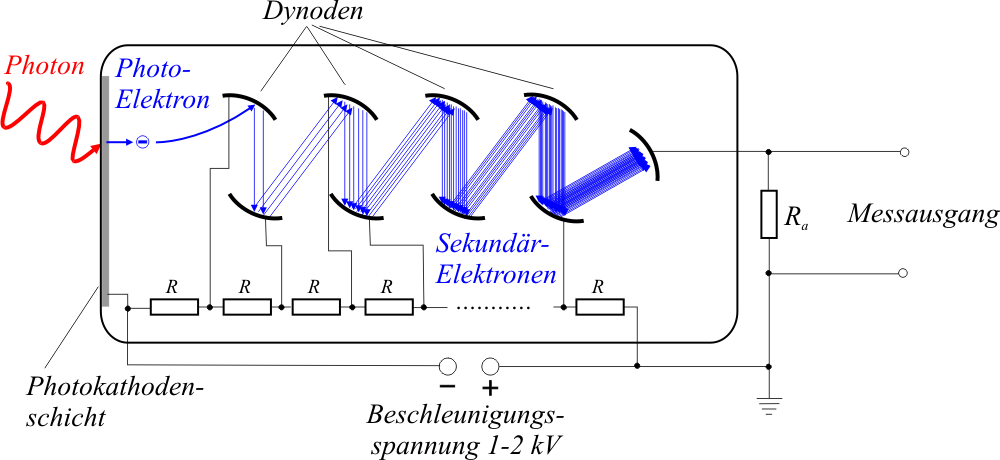
\includegraphics[width=0.85\textwidth]{images/Photomultiplier_schema_de.png}
	\caption{Schematik Photoelektronenvervielfacher}
	\label{theorie_PEV}
\end{figure}

Dort werden durch das Szintillationsphoton Elektronen aus einer Photokathode ausgeschlagen, durch angelegte Spannung zur ersten Dynode beschleunigt wo sie mit der gewonnenen kinetischen Energie weitere Elektronen auschlagen. Dieser Prozess wird einige male wiederholt bis ein messbarer elektrischer Impuls an der Anode entstehen kann.

\subsubsection{Compton-Streuung}

\subsection{Weitwinkel-Compton-Koinzidenz-Methode}

\section{Versuchsaufbau}
Eine Schematische Zeichnung der DREAMS-Anlage ist in Abb. \ref{Auswertung_Bild_DREAMS} zu finden.
\begin{figure}[ht]
	\centering
    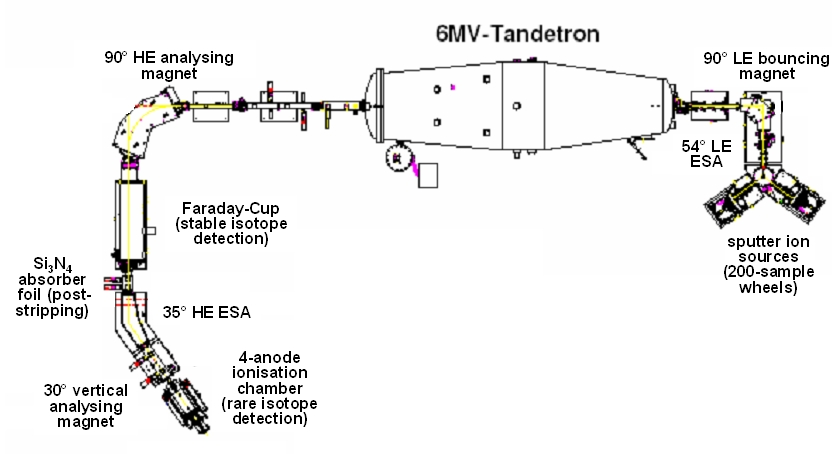
\includegraphics[width=0.85\textwidth]{Pictures/DREAMS.png}
	\caption{Schematik DREAMS \cite{Bild_DREAMS}}
	\label{Auswertung_Bild_DREAMS}
\end{figure}
Sie besteht aus folgenden Komponenten:
\begin{itemize}
    \item Sputter-Ionenquelle
    \item \ang{54} elektrostatischer Analysierer auf der Niederenergieseite
    \item \ang{90} Ablenkmagnet auf der Niederenergieseite
    \item \SI{6}{\mega\electronvolt} Tandem-Beschleuniger
    \item \ang{90} Ablenkmagnet auf der Hochenergieseite
    \item Faraday-Cups zur detektierung stabiler Isotope
    \item SiN Absorberfolie
    \item \ang{35} elektrostatischer Analysierer auf der Hochenergieseite
    \item \ang{30} vertikaler Analysemagnet
    \item Ionisationskammer mit 4 Anoden
\end{itemize} % weitere erklärungen?

\section{Experimenteller Teil}
Im ersten Teil der Auswertung verfolgen wir im Wesentlichen Ionen durch die Anlage.
Untersucht werden soll dabei eine vorbereitete BeO-Probe.
Im zweiten Teil betrachten wir aufgenommene Spektren und untersuchen eine unbekannte Probe.

\subsection{Auf dem Weg zum Beschleuniger}
Nach der Produktion der negativen Ionen durch sputtern werden diese direkt mit insgesamt \SI{29}{\kilo\electronvolt} beschleunigt.
Sie durchlaufen dann eine elektrostatischen Analysierer und einen ersten Ablenkmagneten.
Das Ziel hier ist eine Ionenmasse vorzuselektieren.
Da wir BeO untersuchen sind mögliche gesuchte Ionen $^{9}\text{Be}^{16}\text{O}^{-}$ (stabiles Beryllium-Iosotop) und $^{10}\text{Be}^{16}\text{O}^{-}$ (radioaktives Beryllium-Iostop mit einer Halbwertszeit von \num{1.51e6} Jahren).
Wir kennen die kinetische Energie $E_{\text{kin}}$, den Ladungszustand $q_{\text{ion}}$, die Masse der Ionen $m_{\text{ion}}$ und den Krümmungsradius der weiterführenden Trajektorie $\rho$.
Daher kann man durch geeignete Wahl der Stärke des Magnetfeldes die Ionenmasse auswählen:
\begin{gather}
    B \rho = \frac{p_{\text{ion}}}{q_{\text{ion}}} = \frac{\sqrt{2m_{\text{ion}}E_{\text{kin}}}}{q_{\text{ion}}}
    \label{Auswertung_eq_Magnet}
\end{gather}
Ionen mit einer anderen Masse oder anderem Ladungszustand haben im Magneten eine anders gekrümmte Trajektorie und gelangen daher nicht durch die Eintrittsöffnung zum Beschleuniger.
(Tatsächlich lässt sich wie in Gleichung \ref{Auswertung_eq_Magnet} zu sehen nur nach $\frac{\sqrt{m_{\text{ion}}}}{q_{\text{ion}}}$ selektieren.
Ionen mit vierfacher Masse und doppelter Ladung würden also auch weiterkommen. Derart schwere Teilchen sind jedoch fast gar nicht in der Probe vorhanden.)
Nicht unterscheiden lässt sich jedoch zwischen Molekularen isobaren, so zum Beispiel zwischen $^{10}\text{Be}^{16}\text{O}^{-}$ und $^{9}\text{Be}^{17}\text{O}^{-}$ (wobei $^{17}\text{O}$ in der Natur sehr selten vorkommt) oder $^{10}\text{Be}^{16}\text{O}^{-}$ und $^{10}\text{B}^{16}\text{O}^{-}$ ($^{10}\text{B}$ entsteht beim Beta-Zerfall von $^{10}\text{Be}$).
Für $\rho$ war ein Wert von \SI{0.4}{\metre} gegeben.
Damit ergeben sich für einfach negativ geladene Ionen folgende benötigte Magnetfeldstärken:
\begin{table}[h]
  \centering
  \begin{tabular}{|c|c|}
    \hline
    Ion & Magnetfeldstärke \\
    \hline
    $^{9}\text{Be}^{16}\text{O}^{-}$ & \SI{-0.306}{\tesla} \\
    \hline
    $^{10}\text{Be}^{16}\text{O}^{-}$ & \SI{-0.313}{\tesla} \\
    \hline
  \end{tabular}
  \caption{Benötigte Magnetfeldstärken im ersten Ablenkmagneten für Ionen vor dem Beschleuniger}
  \label{Auswertung_tab_Ionenenergien_vor_Besch}
\end{table}
Um diese Magnetfelder anzulegen ist eine Kalibrierung des Magneten erforderlich, die jedoch in diesem Versuch nicht durchgeführt wurde.
Unsicherheiten der Beschleunigungsspannungen und des Spulenradius werden hier nicht betrachtet, da sie gegenüber der variablen Hysterese des Magneten kaum einen Einfluss auf die Unsicherheit der Ablenkung haben.
Diese wiederrum wäre ebenfalls am besten experimentell (z.B. mittels Hall-Sonde) zu bestimmen.

\subsection{Teilchenenergien nach dem Beschleuniger}
Die Vorselektierten Ionen werden im ersten Teil des Beschleunigers mit der angelegten Spannung beschleunigt.
In der Mitte treffen sie auf Argon an welchem sie sich umladen und die Moleküle aufbrechen.
(Das Aufbrechen der Moleküle ist kein Problem, da chemische Bindungsenergien typischerweise im \si{\electronvolt}-Bereich liegen, die Ionen bis dahin aber schon mehrere \si{\mega\electronvolt} an kinetischer Energie haben.)
Die entstandenen Ionen werden dann mit ihrer positiven Ladung noch ein weiteres Mal mit der angelegten Spannung beschleunigt.
Daher ergibt sich ihre Energie nach dem Beschleuniger zu:
\begin{gather}
    E_{\text{tot}} = e \cdot (U_{\text{Ionenquelle}} + U_{\text{Beschleuniger}}) \cdot \frac{m_{\text{Ion}^{+}}}{m_{\text{Molekül}^{-}}} + U_{\text{Beschleuniger}} \cdot q_{\text{Ion}^{+}}
\end{gather}
Wobei im erste Summand der Term $\frac{m_{\text{Ion}^{+}}}{m_{\text{Molekül}^{-}}}$ benutzt wird um die anteilige kinetische Energie des entstandenen Ions bis zum Argongas zu beschreiben.
Der zweite Summand beschreibt die Beschleunigung nach dem Argongas.

In unserem Versuch betrug die Spannung des Beschleunigers \SI{5.2479e6}{\volt}.
Damit ergeben sich für entstandene Ionen eine Energie nach dem Beschleuniger von:
\begin{center}
  \begin{tabular}{|c|c|}
    \hline
    Ion & Energie \\
    \hline
    $^{9}\text{Be}^{1+}$ & \SI{7.1}{\mega\electronvolt} \\
    $^{9}\text{Be}^{2+}$ & \SI{12.3}{\mega\electronvolt} \\
    $^{9}\text{Be}^{3+}$ & \SI{17.6}{\mega\electronvolt} \\
    $^{9}\text{Be}^{4+}$ & \SI{22.8}{\mega\electronvolt} \\
    \hline
    $^{10}\text{Be}^{1+}$ & \SI{7.3}{\mega\electronvolt} \\
    $^{10}\text{Be}^{2+}$ & \SI{12.5}{\mega\electronvolt} \\
    $^{10}\text{Be}^{3+}$ & \SI{17.8}{\mega\electronvolt} \\
    $^{10}\text{Be}^{4+}$ & \SI{23.0}{\mega\electronvolt} \\
    \hline
    $^{16}\text{O}^{1+}$ & \SI{8.5}{\mega\electronvolt} \\
    $^{16}\text{O}^{2+}$ & \SI{13.7}{\mega\electronvolt} \\
    $^{16}\text{O}^{3+}$ & \SI{19.0}{\mega\electronvolt} \\
    $^{16}\text{O}^{4+}$ & \SI{24.2}{\mega\electronvolt} \\
    \hline
  \end{tabular}
  \captionof{table}{Ionenenergien nach dem Beschleuniger für ausgewählte Ionen}
  \label{Auswertung_tab_Ionenenergien_nach_Besch}
\end{center}

\subsection{Faraday-Cups}
Nachdem wir nun Ionen mit hoher Geschwindigkeit nach dem Beschleuniger haben können wir versuchen häufig auftretende Nuklide nachzuweisen.
Aufgrund der hohen Anteile dieser Nuklide im Telichenstrahl entsteht durch sie ein nennenswerter Ladungsstrom der mit sogenannten Faraday-Cups gemessen werden kann.
Um einzelne Ionsorten detektieren zu können ist nach dem Beschleuniger ein \ang{90} Ablenkmagnet angebracht, der funktioniert wie der auf der Niederenergieseite.
Auch hier ist die Kalibrierung des Magneten uns nicht bekannt.
Im Faraday-Cup werden dann die auftreffenden Ströme gemessen, die bei einem bestimmten Strom durch die Spule durch die abgelenkten Ionen entsteht.
Zunächst wollen wir sehen ob sich die Nuklide unserer BeO-Probe nachweisen lassen.
Dafür wurde in Abb. \ref{Auswertung_Bild_Faraday_Cup_BeO_HE} die gemessenen Ionenströme über dem Strom durch den Ablenkmagneten aufgetragen.
\begin{figure}[ht]
	\centering
    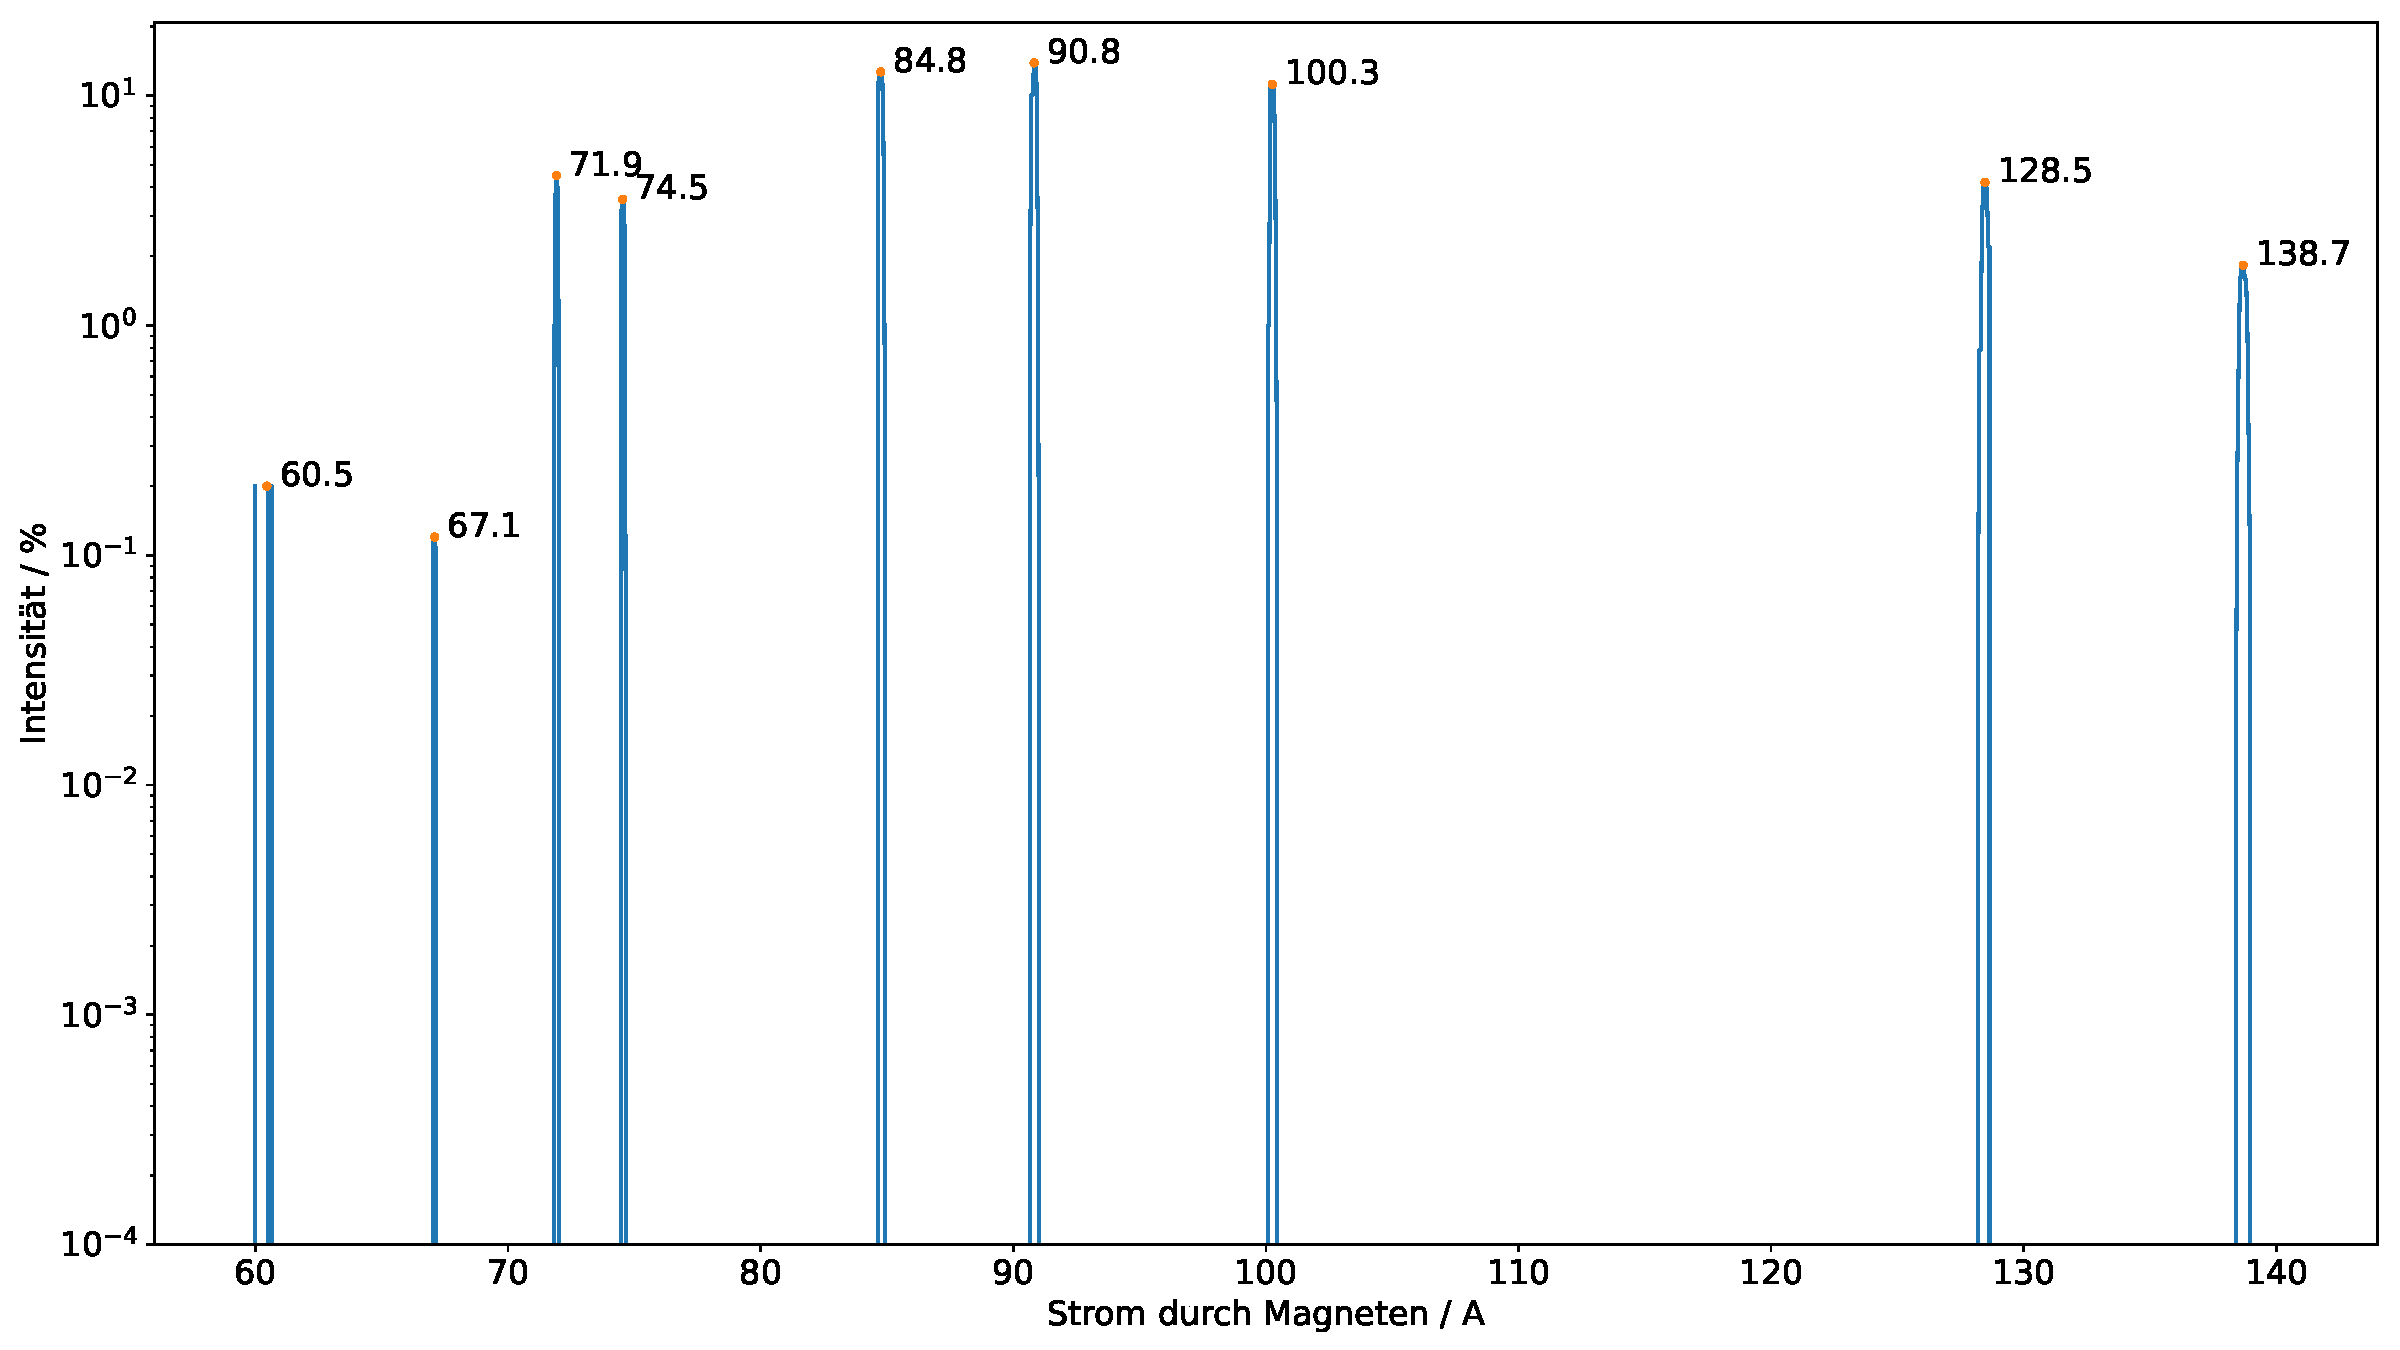
\includegraphics[width=0.85\textwidth]{Pictures/Faraday_Cup_BeO_HE.pdf}
	\caption{Strom gemessen im Faraday-Cup bei variieren des Magnetfeldes auf der Hochenergieseite für BeO-Probe. Die gemittelten x-Werte der Peaks sind eingezeichnet. Die Peaks wurden durch Vergleich mit umliegenden Werten gefunden. Die genaue Position wurde dann ermittelt indem die umliegenden Werte mit ihren Intensitäten als Wichtung gemittelt wurden.}
	\label{Auswertung_Bild_Faraday_Cup_BeO_HE}
\end{figure}
Wäre die Kalibrierung des Magneten bekannt könnte man mithilfe von Formel \ref{Auswertung_eq_Magnet} einfach auf mögliche Ionenspezies bei jedem Peak schließen.
Da dies leider nicht der Fall ist muss man die Peaks untereinander vergleichen.
Mithilfe von Formel \ref{Auswertung_eq_Magnet} wird sofort klar, dass das variieren des Magnetfeldes die Teilchen nur proportional zu $\frac{\sqrt{m_{\text{ion}}}}{q_{\text{ion}}}$ sortieren kann.
Daher kann der relative Abstand der Peaks entlang der x-Achse Aufschluss über die Ionenspezies geben.
Dafür ist es jedoch notwendig zu wissen, welche Ionen man im Ionenstrahl möglicherweise erwartet.
Für die BeO-Probe wurden folgende Ionen für möglich erachtet:
\begin{center}
  \begin{tabular}{|c|c|c|c|}
    \hline
    Element & Masse $/\ \si{\atomicmassunit}$ & Ladungszustand $/\ e$ & $\frac{\sqrt{m_{\text{ion}}}}{q_{\text{ion}}}$\\
    \hline
    \multirow{8}*{Be}    & \multirow{4}*{$9$}  & $1+$                & \num{3}             \\
                         &                     & $2+$                & \num{1.5}           \\
                         &                     & $3+$                & \num{1}             \\
                         &                     & $4+$                & \num{0.75}          \\
    \cline{2-4}
                         & \multirow{4}*{$10$} & $1+$                & \num{3.16}          \\
                         &                     & $2+$                & \num{1.58}          \\
                         &                     & $3+$                & \num{1.05}          \\
                         &                     & $4+$                & \num{0.79}          \\
    \hline
    \multirow{4}*{O}     & \multirow{4}*{$16$} & $1+$                & \num{4}             \\
                         &                     & $2+$                & \num{2}             \\
                         &                     & $3+$                & \num{1.33}          \\
                         &                     & $4+$                & \num{1}             \\
    \hline
    \multirow{4}*{Al}    & \multirow{4}*{$26$} & $1+$                & \num{5.10}          \\
                         &                     & $2+$                & \num{2.55}          \\
                         &                     & $3+$                & \num{1.70}          \\
                         &                     & $4+$                & \num{1.27}          \\
    \hline
  \end{tabular}
  \captionof{table}{Mögliche Ionen auf Hochenergieseite für BeO-Probe.}
  \label{Auswertung_tab_moegl_ionen}
\end{center}
Dabei ist zu beachten das $^{10}\text{B}$ nicht von $^{10}\text{Be}$ unterschieden werden kann, und es daher auch keinen Sinn macht es mit aufzunehmen.
Isobare können erst im weiteren Verlauf getrennt werden.
Aluminium wurde aufgenommen, da es eine häufige Unreinheit in natürlich vorkommendem BeO ist, die ebenfalls zur Altersbestimmung genutzt werden kann.
Außerdem ist $^{26}\text{Al}$ in der Vorselektion nicht vom molekularen Isobar $^{10}\text{Be}^{16}\text{O}$ zu unterscheiden.
Man kann nun versuchen Permutationen dieser Ionen den Peaks zuzuordnen.
Davon gibt es $\frac{n!}{(n-r)!}$ wobei $n$ die Anzahl der möglichen Ionenspezies und $r$ die Anzahl der Peaks sind.
Das sind für $16$ Ionenspezies und $9$ Peaks über $4$ Milliarden.
Es genügt aber natürlich nur Permutationen zuzulassen, bei denen die Ionen nach steigendem $\frac{\sqrt{m_{\text{ion}}}}{q_{\text{ion}}}$ sortiert steigenden Strömen durch den Magneten zugeordnet werden.
Damit reduziert sich die Anzahl der Permutationen auf $\frac{n!}{r! \cdot (n-r)!}$.
Das sind für $16$ Ionenspezies und $9$ Peaks nur noch $11440$, also eine mit einem Computer in sinnvoller Zeit überprüfbare Anzahl.
Mithilfe geeigneter Normen (siehe Appendix \ref{Appendix_Normen}) lassen sich dann die Permutationen finden, die die Peaks am besten beschreiben.
Damit erhält man folgende Permutation als best-passende:
\begin{center}
  \begin{tabular}{|c|c|c|}
    \hline
    Peak $/\ \si{\ampere}$ & Peak-Intensität $/\ \%$ & Ion \\
    \hline
    \num{60.5} & \num{0.2} & $^{10}\text{Be}^{4+}$ \\
    \hline
    \num{67.1} & \num{0.1} & $^{16}\text{O}^{4+}$ \\
    \hline
    \num{71.9} & \num{4.5} & $^{9}\text{Be}^{3+}$ \\
    \hline
    \num{74.5} & \num{3.5} & $^{10}\text{Be}^{3+}$ \\
    \hline
    \num{84.8} & \num{12.7} & $^{26}\text{Al}^{4+}$ \\
    \hline
    \num{90.8} & \num{13.9} & $^{16}\text{O}^{3+}$ \\
    \hline
    \num{100.3} & \num{11.2} & $^{9}\text{Be}^{2+}$ \\
    \hline
    \num{128.5} & \num{4.2} & $^{26}\text{Al}^{3+}$ \\
    \hline
    \num{138.7} & \num{1.8} & $^{16}\text{O}^{2+}$ \\
    \hline
  \end{tabular}
  \captionof{table}{Zuordnung der Teilchenspezies zu den Peaks im Faraday-Cup bei variieren des Magnetfeldes auf der Hochenergieseite für BeO-Probe. Die Abweichung der Verhältnisse für gemessene / erwartete Peakpositionen mit euklidischer Norm ist \num{0.32} (Wurzel des Residuums bei Methode der kleinsten Fehlerquadrate)}
  \label{Auswertung_tab_Teilchenspezies_BeO_HE}
\end{center}
Die Intensitäten der Peaks wurden bisher noch gar nicht beachtet.
Erstaunlich ist der hohe Anteil an Aluminium.
Da wir eine chemisch reine Probe benutzt haben sollte das Aluminium nicht von dieser stammen.
Es ist möglich, dass es von Bauteilen der Anlage stammt, aus denen es von anderen Ionen herausgeschlagen wurde.

\subsection{Isobarentrennung}
Wie in dem vorherigen Abschnitt bereits erwähnt ist es bis hierhin noch nicht möglich gewesen Isobare zu unterscheiden.
Um Abhilfe zu schaffen ist im weiteren Strahlenverlauf eine dünne Schicht aus Siliziumnitrid angebracht.
Da der Verlust an kinetischer Energie von Atomen in Materie stark von der Kernladungszahl abhängt erlaubt dies die Isobarentrennung.
den Faktor $\frac{\Delta E}{\Delta x}$ erhalten wir aus der frei verfügbaren Software SRIM.
Für $^{10}\text{Be}$ ist $\left (\frac{\Delta E}{\Delta x}\right )_{^{10}\text{Be}} = \SI{766.7}{\kilo\electronvolt\per\micro\metre}$.
Die SiN-Folie hat eine Dicke von \SI{1}{\micro\metre}.
Damit ergibt sich ein Energieverlust der $^{10}\text{Be}$-Atome von \SI{766.7}{\kilo\electronvolt}.
Die verbleibende Energie der $^{10}\text{Be}$-Ionen ist dann, abhängig von deren Energie vorher:
\begin{center}
  \begin{tabular}{|c|c|c|}
    \hline
    Ion & Energie nach Beschleuniger & Energie nach Folie \\
    \hline
    $^{10}\text{Be}^{1+}$ & \SI{7.3}{\mega\electronvolt}  & \SI{6.5}{\mega\electronvolt}  \\
    $^{10}\text{Be}^{2+}$ & \SI{12.5}{\mega\electronvolt} & \SI{11.6}{\mega\electronvolt} \\
    $^{10}\text{Be}^{3+}$ & \SI{17.8}{\mega\electronvolt} & \SI{17.0}{\mega\electronvolt} \\
    $^{10}\text{Be}^{4+}$ & \SI{23.0}{\mega\electronvolt} & \SI{22.3}{\mega\electronvolt} \\
    \hline
  \end{tabular}
  \captionof{table}{Ionenenergien nach ser SiN Folie in Abhängigkeit der Ladungszustände aus dem Beschleuniger.}
  \label{Auswertung_tab_Ionenenergien_nach_Folie}
\end{center}
Nach der Folie wird $^{10}\text{Be}$ nur noch im Ladungszustand $4+$ erwartet, da die Atome durch die Foile weiter ionisiert werden.

Um nun die Isobare $^{10}\text{Be}$ und $^{10}\text{B}$ zu trennen ist nach der Folie ein elektrostatischer Analysierer angebracht.
Die Spannung die angelegt werden muss kann berechnet werden durch Kräftegleichgewicht:
\begin{gather}
    q_{\text{Ion+}} \cdot \frac{U_{\text{Platte}}}{d_{\text{Platte}}} = \frac{mv^{2}}{r}
\end{gather}
Wobei $d_{\text{Platte}} = \SI{3.6}{\centi\metre}$ und $r = \SI{2.6}{\metre}$ ist.
Die Spannung, die einzustellen ist, ist jedoch nur die halbe, da auf den Platten jeweils $+U_{\text{Platte}}$ und $-U_{\text{Platte}}$ erzeugt wird (die Spannung wird beim einstellen relativ zur Erdung gemessen).
Für das Ion $^{10}\text{Be}^{4+}$ ergibt sich daher in Abhängigkeit der Energie nach der Folie eine Ablenkspannung von:
\begin{center}
  \begin{tabular}{|c|c|c|}
    \hline
    Ion & Energie nach Folie & $\frac{U_{\text{Platte}}}{2}$ \\
    \hline
    \multirow{4}*{$^{10}\text{Be}^{4+}$} & \SI{6.5}{\mega\electronvolt}  & \SI{22.5}{\kilo\volt} \\
                                         & \SI{11.6}{\mega\electronvolt} & \SI{40.7}{\kilo\volt} \\
                                         & \SI{17.0}{\mega\electronvolt} & \SI{58.9}{\kilo\volt} \\
                                         & \SI{22.3}{\mega\electronvolt} & \SI{77.0}{\kilo\volt} \\
    \hline
  \end{tabular}
  \captionof{table}{Ablenkspannug für den ESA für verschiedene Ionenenergien.}
  \label{Auswertung_tab_Ablenkspannung_ESA}
\end{center}


\nocite{*} % alle resourcen auflisten
\printbibliography

\appendix
\section{Spezieszuordnung}
\label{Appendix_Normen}
Mithilfe einer Norm lassen sich die Permutationen von Ionenspezies bestimmen, die die Peaks im Faraday-Cup am besten beschreiben.
Zuerst wurden die gemessenen Magnetstromstärken-Peaks $\vec{P}_{\text{exp}}$ ermittelt.
Aus diesen wurden die Verhältnisse $\vec{r}_{\text{exp}}$ gebildet.
Dann wurde für die möglichen Ionenspezies $\vec{P}_{\text{möglich}}$ in der Probe das Verhältnis $\frac{\sqrt{m_{\text{ion, möglich}}}}{q_{\text{ion, möglich}}}$ gebildet.
Die Ionenspezies wurden nach diesem Verhältnis geordnet und die erwähnten, geordneten Permutationen $\vec{\nu}(k)$ gebildet.
(Nur Permutationen in dem die Reihenfolge der Elemente nicht vertauscht wird, aber Elemente weggelassen werden können.)
Für diese Permutationen wurde dann ebenfalls das Verhältnis $\vec{r}_{\text{möglich}\ \nu_{i}(k)}$, diesmal von $\frac{\sqrt{m_{\text{ion, möglich}}}}{q_{\text{ion, möglich}}}$, erstellt.
(Das ist ein Vektor für jede Permutation.)
Dann wurde mithilfe der euklidischen Norm der \glqq Abstand\grqq{} der Verhältnisse gebildet:
\begin{gather}
    \norm{\vec{r}_{\text{exp}}-\vec{r}_{\text{möglich}\ \nu_{i}(k)}} = \sqrt{\sum_{n}(\vec{r}_{\text{exp}\ n}-\vec{r}_{\text{möglich}\ \nu_{i}(k),n})^{2}}
\end{gather}
(In Anlehnung an die Methode der kleinsten Fehlerquadrate. Man könnte die Wurzel auch weglassen. Da die Wurzelfunktion monoton ist ändert sie die Reihenfolge später nicht.)
Die Permutation mit der kleinsten Norm ist dann gerade die beste Zuordnung der Ionenspezies zu den Peaks.


% ----- DOKUMENT ENDE -----

\end{document}
